En este capítulo se revisarán las aplicaciones y estudios hechos en el área.
Para ordenar esta sección, se dividirá respecto a los métodos cuantitativos a
usar (neural-wavelet), sus aplicaciones en esta área, y finalmente los
desarrollos realizados mediante técnicas de HPC.

\section{Redes Neuronales Artificiales}

Las redes neuronales artificiales (ANN), han sido usadas en distintos campos de
la ciencia, en particular en el área de computación, ya que son de interés como
herramienta para procesos de minería de datos \cite{bigus1996data}. Se ha
convertido en una metodología multipropósito, robusta computacionalmente, con
apoyo teórico sólido. Los problemas de minería de datos no son de naturaleza
computacional generalmente, sino que son técnicas o metodologías, para
satisfacer algún tipo de apoyo a procesos que involucren manejo con grandes
volúmenes de datos. Los modelos de redes neuronales buscan encontrar relaciones
entre los datos existentes, la manera en que lo hacen es de forma inductiva, es
decir, mediante algoritmos de aprendizaje.

Una neurona aritificial es un procesador elemental (PE), que recibe una serie
de entradas con pesos diferentes, las procesa y proporciona una salida única. A
cada neurona llegan muchas señales de otras, proceso conocido en la biología
como Sinapsis, y producen una única salida (Axon). Una sinapsis que comunica dos
neuronas puede ser de naturaleza excitadora o inhibidora. En el primer caso, la
neurona emisora tenderá a activar a la neurona receptora, y en el segundo caso,
la neurona emisora tenderá a inhibir la actividad de la neurona receptora.

Cada sinapsis se caracteriza además por la eficacia con la que se establece la
conexión. Aunque la neurona toma dediciones en función de la suma de
información que recibe, la contribución de cada una de estas informaciones que
recibe es ponderada por la eficacia de la sinapsis correspondiente.

La primera neurona artitificial fue concebida por W. McChulloch, y W. Pitts. Se
trata de un modelo binario cuyo estado es 1 (activo) o 0 (inactivo).
Periódicamente actualiza su estado calculando la suma de sus entradas con el
valor de cada entrada modulado por la eficacia sináptica correspondiente, y
toma una decisión comparando esta suma con un cierto nivel fijado. Si la suma
es superior al umbral, la neurona se activa, y en caso contrario inactiva. Por
tanto, todas las neuronas toman sus decisiones simultáneamente tendiendo en
cuenta la evolución del estado global de la red. La función de activación
corresponde a una función no lineal. El modelo queda como:


$$ y = \gamma \left( \sum_{i = 1}^{m}w_ix_i + w_0 \right) $$

Donde:
\begin{itemize}
	\item $w_i$: pesos de la entrada i o eficacia de la sinapsis.
	\item $x_i$: entrada i.
	\item $w_o$: sesgo.
	\item $\gamma$: función no lineal.
\end{itemize}

La propuesta de McCulloch fue una salida binaria $sign(z)$, es decir:

$$ \gamma(z) = sign(z) = \left\{
	       \begin{array}{ll}
		 1      & \mathrm{si\ } z \ge 0 \\
		 -1	& \mathrm{si\ } z < 0  \\
	       \end{array}
	     \right. $$

Esta no es la única función no lineal que se puede especificar.

Una red neuronal es un set de PE interconectados entre si, imitando la
actividad del cerebro. La siguiente figura muestra una neruna dentro de una red
neuronal:

\begin{figure}[h!t]
    \begin{center}
        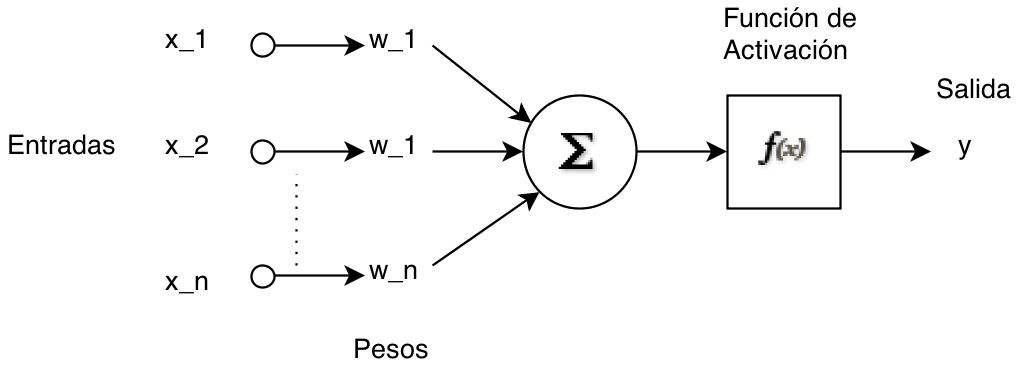
\includegraphics[width=0.4\textwidth]{images/ann_model}
        \caption{Modelo de neurona artificial.}
    \end{center}
\end{figure}

En la figura, cada uno de las entradas $x_i$ tiene un peso $w_i$ que representa
la fuerza de esa conexión en particular. La suma de esas entradas pesadas son
la entrada para la función de activación que genera la salida.

\subsection{Tipos de aprendizaje}

Una de las principales capacidades de una ANN es su capacidad de aprender a
partir de un conjunto de patrones de entrenamiento, es decir, que es capaz de
encontrar un modelo de ajustes de dato. Es por ello que se conocen varios tipos
de aprendizajes:

\subsubsection{Aprendizaje supervisado}

El aprendizaje supervisado es un caso de entrenamiento con entrenador, y se
utiliza información global. En su implementación se presentan dos vectores (uno
de entrada y otro de salida deseada).  La salida computada por la red se
compara con la salida deseada, y los pesos de la red se modifican en el
sentido de reducir el error cometido. Se repite iterativamente, hasta que la
diferencia entre la salida computada y la deseada sea aceptablemente pequeña,
comparada con algún parámetro de error. Con \emph{n} parejas de este tipo se
forma un conjunto de entrenamiento.

El aprendizaje supervisado se suele dividir a su vez en dos sub categorías:
\begin{itemize}
	\item[-] Aprendizaje estructural: se refiere a la búsqueda de la mejor 
conexión o afinidad posible entrada/salida para cada paerja de patrones 
individuales. Este enfoque es uno de los más utilizados
	\item[-] Aprendizaje temporal: hace referencia a la captura de una serie 
	de patrones necesarios para conseguir algún resultado final. En el aprendizaje 
	temporal la respuesta actual de la red depende de las entradas y respuestas 
	previas. En el aprendizaje estructural no existe esta dependencia.
\end{itemize}

\subsubsection{Aprendizaje no supervisado}

El aprendizaje no supervisado es un caso de entrenamiento sin entrenador y sólo
se usa información local durante todo el proceso de aprendizaje. Es un modelo
más cercano al sistema biológico, no se utiliza vector de salida esperada, y
sólo hay vectores de entrada en el conjunto de entrenamiento. El algoritmo
modifica los pesos de forma que las salidas sean consistentes, es decir, que a
entradas muy parecidas, la red compute la misma salida.  Las salidas se asocian
a las entradas de acuerdo con el proceso de entrenamiento. El proceso extrae
características, abstrayendo las propiedades colectivas subyacentes del
conjunto de entrenamiento, y agrupa por clases de similitudes.

\subsubsection{Aprendizaje Hebbiano}

El aprendizaje Hebbiano propone que los pesos de la red se incrementan si las
neuronas origen y destino están activadas, es decir, refueza los caminos usados
frecuentemente en la red, lo que explicaría los hábitos y el aprendizaje por
repetición.

El aprendizaje hebbiano está matemáticamente caracterizado por la ecuación:

$$ w_{ij}^{nuevo} = w_{ij}^{anterior} + a_{ki}b_{kj} $$

Donde $i = 1,2,...,n$; $j=1,2,...,p$; $w_{ij}$ es el peso de la conexión entre
los dos procesadores elementales (neuronas artificiales).

Las redes neuronales como la memoria asociativa lineal emplean este tipo de
aprendizaje. El número de patrones que una red adiestra usando conexiones y
pesos ilimitados puede producir, está limitado por la dimensión de patrones de
entrada.

Si los valores de los PEs están limitados y los pesos ilimitados, se encuentra
el caso denominado Hopfield, que restringen el valor de los PEs a un valor
binario o bipolar.  

%\subsubsection{Aprendizaje competitivo}
%
%El aprendizaje competitivo usa inhibición lateral para activar una sola neurona
%(se puede ver como el ganador). Algunas redes neuronales que emplean
%aprendizaje competitivo son los mapas auto-organizativos (Kohonen,1984) y
%Adaptive Resonanse Theory (Caprenter y Grossber).

\subsubsection{Aprendizaje Min-Max}

Un clasificador min-max usa un par de vectores para cada clase. La clase
\emph{j} está representada por el PE $y_i$ y está definida por los vectores
$V_j$ (el vector min) y $W_j$ (el vector max).  El aprendizaje min-max es un
sistema neuronal que viene dado por la ecuación:

$$ v_{ij}^{nuevo} = min(a_{ki},v_{ij}^{anterior}) $$

para el vector min y:

$$ w_{ij}^{nuevo} = min(a_{ki},w_{ij}^{anterior}) $$

\subsubsection{Aprendizaje de correción de error}

Este tipo de aprendizaje ajusta los pesos de conexión entre PEs en proporción a
la diferencia entre los valores deseados y los computados para cada PE de la
capa de salida. Dependiendo del número de apas de las redes se distinguen dos
casos:
\begin{itemize}
	\item[-] Red de dos capas: puede capturar mapeos lineales entre las entradas 
	y salidas. DOs redes neuronales que utilizan este tipo de aprendizaje son el 
	Perceptrón (Rosenblatt) y ADALINE (Widrow y Hoff)
	\item[-] Red multicapa: peden capturar mapeos no lineales entre las entradas 
	y salidas. La versión multinivel de este algoritmo es denominado Regla de 
	Aprendizaje de Retropropagación de errores (Backpropagation). Utilizando la 
	regla encadenada, se calculan los cambios de los pesos para un número arbitrario 
	de capas. El número de iteraciones que deben ser realizadas para cada patrón 
	del conjunto de datos es grande, haciendo este algoritmo de aprendizaje muy 
	lento para entrenar. El algoritmo de retropograpagión ha sido estudiado por 
	Werbos (1974) y Parker (1982), y fue introducido por Rumerlhart, Hilton y 
	Williams (1986).
\end{itemize}

\subsubsection{Aprendizaje reforzado}

Esta heurística para redes neuronales fue ideada por Widrow, Gupta y Maitra
(1973) y desarrollado por Williams (1983). Este tipo de aprendizaje es similar
al anterior, en que los pesos son fortalecidos en las acciones desarrolladas
correctamente y penalizados en aquellas mal realizadas. La diferencia entre ambas
es que el aprendizaje por correción de error utiliza información de error más
específica reuniendo valores del error por cada PE de la capa de salida,
mientras que el aprendizaje reforzado utiliza información de error no
específica para determinar el desarrollo de la red. Mientras que el primero
tiene un vector completo de valores que utiliza para la correción de error,
sólo un valor es usado para describir la ejecución de la capa de salida durante
el aprendizaje reforzado. Esta forma de aprendizaje es ideal en situaciones
donde no está disponible información específica sobre el error, pero sí
información global de la ejecución, tal como predicción y control.

Las redes que implementan este tipo de aprendizaje son: Adaptive Hueristic
Critic, Barto, Sutton y Anderon 1983, y Associative Reward-Penalty, Barto 1985.

\subsubsection{Tabla Resumen}

Una tabla de resumen para recordar los factores e importancia de cada tipo de aprendizaje sería:

\begin{tabularx}{\textwidth}{|X|X|X|X|X|X|}
	\hline 
	Aprendizaje	& Tiempo entrenamiento	& Supervisión			& Linealidad	& Estructural / Temporal	& Cap. de almacen. \\
	\hline 
	Hebbiano 	& Rápido		& No supervisado		& Lineal	& Estructural			& Baja	\\
	Min-Max		& Rápido		& No supervisado		& No lineal	& Estructural			& Buena	\\
	Corr. error dos niveles & Lento		& Supervisado			& Lineal	& Ambos				& Buena	\\
	Corr. error multinivel & Muy lento	& Supervisado			& No lineal	& Ambos				& Alta	\\
	Reforzado	& Muy lento		& Supervisado			& No lineal	& Ambos				& Buena \\
	\hline 	
\end{tabularx}


%\subsection{Feedforward Artificial Neuronal Network}
%
%El modelo de red neuronal a utilizar en esta memoria, serán las Feedforward
%Artificial Neuronal Network (FFANN).
%
%$$ g_{\lambda}(x,w) = \gamma_2 \left( \sum_{j = 1}^{\lambda} w_j^{[2]} \gamma_1 
%\left( \sum_{i = 1}^{m} w_{ij}^{[1]}x_i + w_{m+1,j}^{[1]} \right) + 
%w_{\lambda+1}^{[2]} \right) $$
%
%En donde:
%\begin{itemize}
%	\item Las principales componentes se mantienen al igual que en el modelo más 
%simple, es decir, $w$ y $x$ siguen siendo los vectores de los pesos y datos de entrada.
%	\item $\gamma_2$: Es una función que puede ser lineal o no.
%	\item $\gamma_1$: Es una función no lineal y diferenciable.
%\end{itemize}
%
%La estructura física de cómo se compone el modelo es una división por capas:
%\begin{itemize}
%	\item Capa de entrada.
%	\item Capa oculta.
%	\item Capa de salida.
%\end{itemize}
%
%Dado un conjunto de observaciones, la tarea del aprendizaje neuronal es construir un estimado $g_{\lambda}(x,w)$ de la función desconocida

\section{Análisis Wavelets}
La teoria de las funciones wavelet fue desarrollada en distintos campos del
conocimiento como las matemáticas, física e ingeniería eléctrica, enfocándose
en el análisis de señal contínua o discreta.

El análisis wavelet consiste en la descomposición de una señal en un conjunto
jerárquico de aproximaciones y detalles. En cada nivel de la jerarquía se
obtiene una señal de aproximación y una señal de detalle, la señal de
aproximación obtenida es una aproximación de la señal original que toma en
cuenta las frecuencias bajas mientras que la señal de detalles corresponde a
los componentes de alta frecuencia. Las wavelets son funciones que permiten
descomponer una señal en distintos componentes de frecuencia y después analizar
cada uno en una resolución acorde a su escala.

\subsection{Análisis de Fourier}
De acuerdo a la teoría de Fourier, una señal puede ser expresada como una suma
de series de senos y cosenos. Esta suma también es llamada la expansión de
Fourier. Sin embargo, uno de los inconvenientes de la transformada de Fourier
es que solamente tiene resolución de frecuencia y no resolución de tiempo. Por
lo tanto, se puede identificar todas las frecuencias presentes en una señal,
pero no se sabe cuando estas están presentes. Para avordar este problema, se propone la teoría de Wavelet:

$$
F(\omega) = \int^{+\infty}_{-\infty} f(t)e^{-jwt} dt
$$

\begin{eqnarray*}
	F(\omega)	&=&	\int^{+\infty}_{-\infty} f(t)e^{-jwt}dt \\
				&=&	\int^{+\infty}_{-\infty} f(t)(\cos\omega t - i\sin\omega t)dt
\end{eqnarray*}

Del punto vista matemático, una wvalet puede ser definida como una función con promedio cero:
\begin{eqnarray*}
	\int^{+\infty}_{-\infty} \psi(t)dt &=& 0 \\
\end{eqnarray*}

La idea básica de la transformada wavelet es representar una función como una
superposición de un set de wavelets o funciones bases. Como estas funciones son
pequeñas ondas ubicadas en diferentes tiempos, esta transformada puede proveer
información acerca de la señan en el dominio del tiempo y frecuencia.

\subsection{Transformada Wavelet Contínua (CWT)}
Similar a la ecuación de la transformada de Fourier, la transformada contínua
wavelet se define como:
\begin{eqnarray*}
	\gamma(s,\tau) = \int^{+\infty}_{-\infty}f(t)\Psi^{*}_{s,\tau}(t)dt
\end{eqnarray*}

Donde * denota una conjugación compleja. Las variables s y $\tau$ son las
nuevas dimensiones: escala y traslación, después de la transformada wavelet.
Esta ecuación muestra como la función $f(t)$ en base a un set de funciones
$\psi_{s,\tau}(t)$ que son llamadas wavelets. Y las wavelets son generadas dese
una wavelet madre escala y trasladada:
\begin{eqnarray*}
	\Psi_{s,\tau}(t) = \frac{1}{\sqrt{s}}\psi\left(\frac{t-\tau}{s}\right)
\end{eqnarray*}

Donse $s$ es un factor de escala, es decir, escala el ancho de una funcion base
en particular, $\tau$ es un factor de traslación que especifica la traslación
de la posición en base al eje t, y finalmente el factor $\frac{1}{\sqrt{s}}$ es
por la normalización de energía a través de diferentes escalas. Como la
transformada de Fourier descompone una señal en una serie de senos y cosenos
con diferentes frecuencias, la trasnformada contínua wavelet descompone una
señal en una serie de wavelets con diferentes escalas y traslaciones.

\subsection{Transformada Wavelet Discreta (DWT)}
La desventaja de la transformada contínua wavelet reside en su complejidad
computacional y redundancia. Para resolver este problema, se introduce la
transformada discreta wavelet. A diferencia de CWT, la DWT descompone la señal en un set de wavelets ortogonales entre si. DWT se define como:
\begin{eqnarray*}
	\psi_{j,k}(t) = \frac{1}{\sqrt{s^{j}_{0}}}\psi\left(\frac{t-k\tau_0s^{j}_{0}}{s^{j}_{0}}\right)
\end{eqnarray*}

Donde $j$ y $k$ son enteros, $s_0 > 1$ es un paso fijo de dilatación y el
factor de $\tau_0$ depende del paso de dilatación. La función de escala y la
función wavelet de DWT se definen como:
\begin{eqnarray*}
	\varphi(2^jt)	&=&	\sum^{k}_{i=1}h_{j+1}(k)\varphi(2^{j+1}t-k)\\
	\psi(2^jt)		&=&	\sum^{k}_{i=1}g_{j+1}(k)\varphi(2^{j+1}t-k)
\end{eqnarray*}

En base a esto, la señal $f(t)$ puede ser expresada como:
\begin{eqnarray*}
	f(t) = \sum^{k}_{i=1}\lambda_{j-1}(k)\varphi(2^{j-1}t-k) + \sum^{k}_{i=1}\gamma_{j-1}(k)\psi(2^{j-1}t-k)
\end{eqnarray*}

La DWT se puede hacer usando el esquema de banco de filtros $cita$. La
siguiente figura muestra el banco de filtros de dos canales para la DWT.

\begin{figure}[h!t]
    \begin{center}
        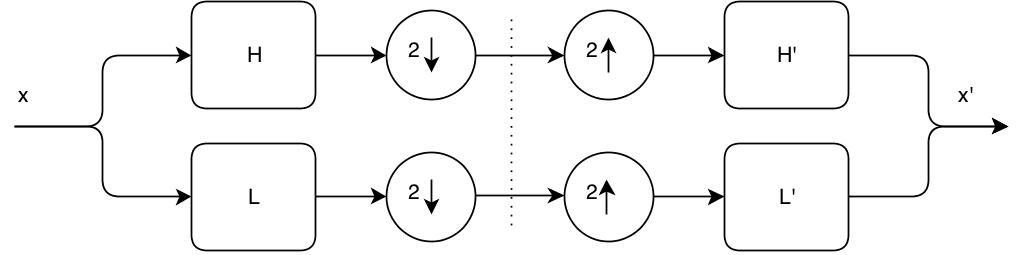
\includegraphics[width=0.7\textwidth]{images/filter_bank}
        \caption{Esquema de banco de filtros para la DWT.}
    \end{center}
\end{figure}

En la figura, H,L y H',L' son los filtros de pasa alto y pasa bajo para la
descomposición wavelet y reconstrucción respectivamente. En la fase de
descomposición, los filtros de pasa bajo remueven los componentes de alta
frecuencia de la señal, y los filtros de pasa alto toman las partes restantes.
Entonces, la señal filtrada es decimada en dos, proceso conocido como
down-sampling, y los resultados son llamados como, coeficientes de aproximación
y los coeficientes de detalle. La reconstrucción es el proceso inverso a la
descomposición y para una reconstrucción de banco de filtros perfecto, se tiene
x = x'. Una señal puede ser descompuesta por el algoritmo piramidal o de cascada:

\begin{eqnarray*}
    x(t)	&=& A_1(t) + D_1(t)\\
			&=& A_2(t) + D_2(t) + D_1(t) \\
			&=& A_3(t) + D_3(t) + D_2(t) + D_1(t)\\
			&=& A_n(t) + D_n(t) + D_{n-1}(t) + ... + D_1)
\end{eqnarray*}

donde $D_n(t)$ y $A_n(t)$ son los coeficientes de detalle y aproximación al
nivel n respectivamente. La siguiente figura representa la descomposición:

\begin{figure}[h!t]
    \begin{center}
        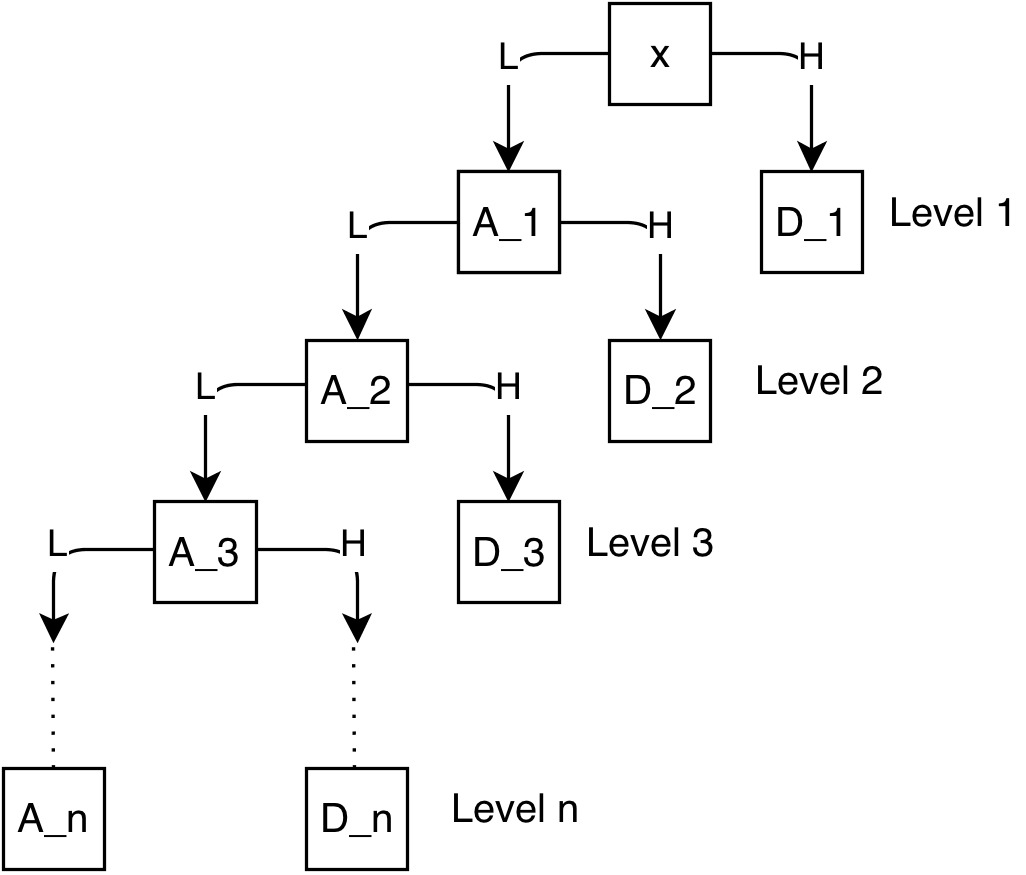
\includegraphics[width=0.4\textwidth]{images/piramidal}
        \caption{Árbol de descomposición piramidal.}
    \end{center}
\end{figure}

\section{Redes neuronales wavelet}
La arquitectura más sencilla de una red neurnal wavelet consiste en tener una
sola entrada y una sola salida. En esta arquitectura la capa oculta está
formada por wavelons cuyos parámetros de entrada están definido por peso,
parámetro de traslación y escalamiento. La salida de la red es una combinación
lineal de funciones wavelet de cada wavelon. La salida de un wavelon con una
entrada sencilla está dada por:

\begin{eqnarray*}
    \Psi_{\lambda,t}(u) = \Psi\left(\frac{u-t}{\lambda}\right)
\end{eqnarray*}

La arquitectura de una red neuronal wavelet se muestra en la siguiente figura,
laca oculta consiste en M wavelons y la capa de salida consiste en un sumador:

\begin{figure}[h!t]
    \begin{center}
        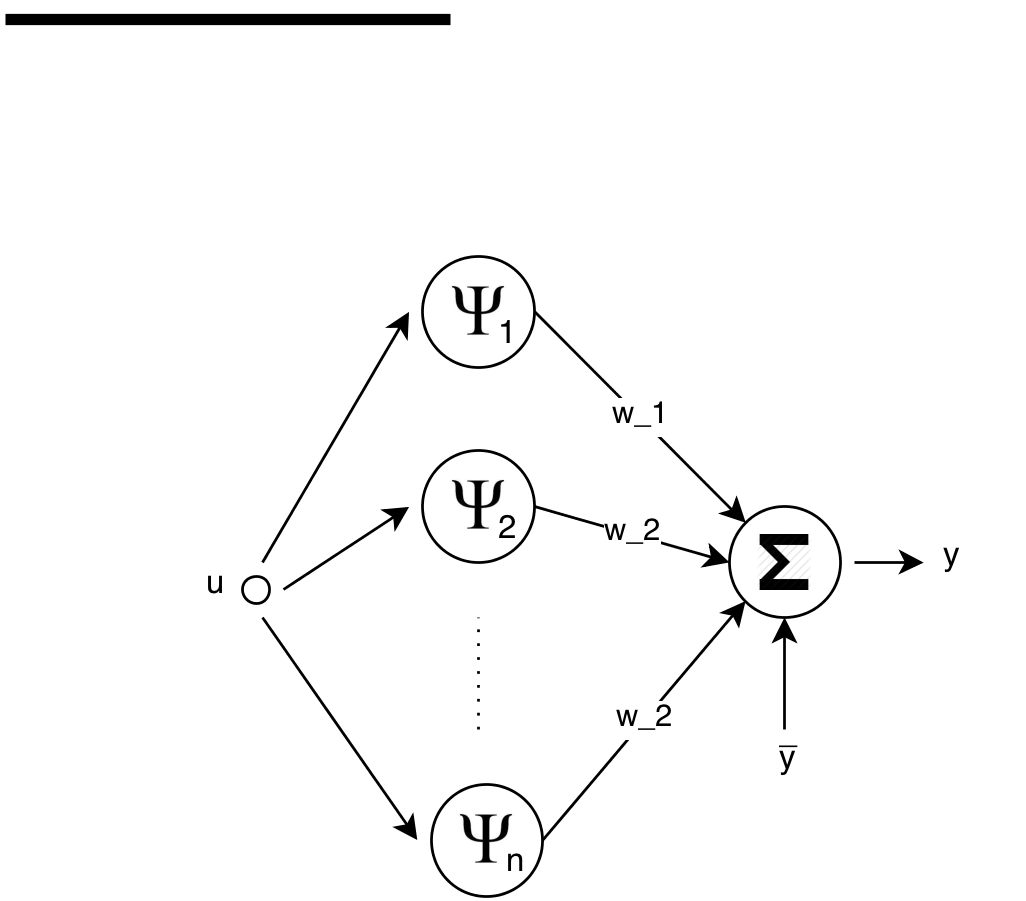
\includegraphics[width=0.4\textwidth]{images/1_in_1_out}
        \caption{Arquitectura de una entrada y una salida.}
    \end{center}
\end{figure}

La salida está dada por:

\begin{eqnarray*}
    y(u) = \sum_{i=1}^{n} w_i\Psi_{\lambda_i,t_i} + \bar{y}
\end{eqnarray*}

\subsection{Wavenet}
La arquitectura de una wavenet es similar a la de la red neuronal wavelet, a
execpción de que los parámetros de traslación y escalamiento se mantienen fijos
desde la inicialización y no son alterados durante el proceso de aprendizaje.
Su salida está dada por:

\begin{eqnarray*}
    y(u) = \sum_{i=1}^{n} w_i\phi_{\lambda_i,t_i} + \bar{y}
\end{eqnarray*}

donde $\phi_{\lambda_i,t_i}$ representa la función de escalamiento y parámetros
de traslación y escalamiento mantienen las restricciones mencionadas
anteriormente.

\section{Computación de Alto Desempeño}
\subsection{Graphic Processing Unit}
\subsection{Computación Heterogenea}
